\section{Phonon-assisted optical absorption}\label{sec:6.5}

Silicon solar cells absorb the whole visible spectrum, from about 1.6 to \SI{3.3}{eV}, and silicon photodiodes respond down to its gap of \SI{1.17}{eV}. Yet the smallest vertical gap of silicon, $E_{\mathrm{dir}}$, is \SI{3.4}{eV} (\cref{sec:3.3}). A photon carries almost no crystal momentum, and on its own it can lift an electron only vertically, from $(v,\vect{k})$ to $(c,\vect{k})$. Every photon that silicon absorbs between \SI{1.17}{} and \SI{3.4}{eV} is therefore absorbed together with a phonon, which carries the crystal momentum $\vect{k}_{\mathrm{c}}$ from the valence maximum at $\mathrm{\Gamma}$ to a conduction valley. The phonon can be created or destroyed, and it takes a few tens of meV from the absorbed energy or adds as much. Phonon-assisted absorption is the simplest composite process: two vertices, the photon's and the electron--phonon vertex $g$ of \cref{sec:6.2}, joined through virtual intermediate states with the energy denominators of \cref{sec:2.4}. An absorbed dark-matter boson has even less momentum for its energy than a photon, and between the indirect and the direct gap it is absorbed only with a phonon (\cref{sec:13.8}). A scattering dark-matter particle just above its threshold mass delivers its energy at momentum transfers too small to reach $\vect{k}_{\mathrm{c}}$, and a phonon again supplies the crystal momentum that the momentum transfer lacks (\cref{sec:13.1}).

\subsection{The optical vertex}

A uniform optical field $\vect{\mathcal{E}}(t) = -\mathcal{E}\,\hat{\vect{e}}_\gamma\cos\omega t$, with unit polarization vector $\hat{\vect{e}}_\gamma$, is described by the vector potential $\vect{A}(t) = (\mathcal{E}/\omega)\,\hat{\vect{e}}_\gamma\sin\omega t$. To first order in $\vect{A}$ the field couples to the electrons through
\begin{equation}
  H_A = e\,\vect{A}\cdot\op{\vect{V}}, \qquad
  \op{\vect{V}} = \sum_{\vect{k}}\sum_{mn}\vect{v}_{mn}(\vect{k})\,c^\dagger_{m\vect{k}}c_{n\vect{k}} ,
  \label{eq:6.5-HA}
\end{equation}
where $\op{\vect{V}}$ is the total velocity of the electrons, written over Bloch states with the velocity matrix elements $\vect{v}_{mn}(\vect{k})$ of \cref{eq:3.2-pv}, and the spin is summed implicitly. For a local potential $\op{\vect{V}} = \sum_j\op{\vect{p}}_j/m_e$, and the sign of the charge is irrelevant for rates. The velocity operator conserves $\vect{k}$, because the velocity commutes with lattice translations. The part of $H_A$ that oscillates as $\ee^{-\ii\omega t}$ absorbs the energy $\omega$, with the amplitude $(e\mathcal{E}/2\omega)\,\hat{\vect{e}}_\gamma\cdot\op{\vect{V}}$ up to a phase.

\Cref{eq:6.5-HA} is the \emph{velocity form} of the optical vertex. Its alternative, the length form $e\vect{\mathcal{E}}\cdot\sum_j\vect{r}_j$, is awkward in a crystal, since the position has no matrix elements between extended Bloch states except through the commutator of \cref{eq:3.2-r}. The velocity form needs just $\vect{v} = \ii[H_{\mathrm{e}},\vect{r}]$, which stays well defined when the potential is nonlocal (\cref{eq:3.2-dHk}). It is also the vertex that dark matter shares with light. By \cref{eq:3.2-optical}, the density vertex at small momentum transfer is $\rho_{mn}(\vect{k},\vect{q}) \to \vect{q}\cdot\vect{v}_{mn}/(\varepsilon_{m\vect{k}} - \varepsilon_{n\vect{k}})$. On the energy shell the denominator is $\omega$, and a longitudinal field coupled through the density and a transverse field coupled through the velocity carry the same matrix element, $\hat{\vect{e}}_\gamma\cdot\vect{v}_{mn}/\omega$. Replacing the photon by dark matter replaces this optical limit by the full density vertex, and nothing else in the structure changes.

At first order the golden rule \cref{eq:2.5-golden} with $H_A$ gives the absorption rate between many-body states $i$ and $f$, and the absorbed power is $\omega$ times the net rate, absorption minus stimulated emission. Equating the time-averaged power per volume with $\sigma_1\mathcal{E}^2/2$ and using $\sigma_1 = \omega\varepsilon_2$ (\cref{eq:4.4-sigma}) gives
\begin{equation}
  \varepsilon_2(\omega) = \frac{\pi e^2}{\omega^2\Vol}\sum_{i,f}(p_i - p_f)\,\bigl|\hat{\vect{e}}_\gamma\cdot\langle f|\op{\vect{V}}|i\rangle\bigr|^2\,\delta(E_f - E_i - \omega) .
  \label{eq:6.5-eps2many}
\end{equation}
For independent electrons at $T \ll \Eg$ the final states are one electron in $(c,\vect{k})$ and one hole in $(v,\vect{k})$, and \cref{eq:6.5-eps2many} is the direct absorption of \cref{sec:4.4}, the familiar sum over vertical transitions,
\begin{equation}
  \varepsilon_2(\omega) = \frac{g_{\mathrm{deg}}\,\pi e^2}{\omega^2 \Vol}\sum_{\vect{k}}\sum_{cv}\bigl|\hat{\vect{e}}_\gamma\cdot\vect{v}_{cv}(\vect{k})\bigr|^2\,\delta(\varepsilon_{c\vect{k}} - \varepsilon_{v\vect{k}} - \omega) ,
  \label{eq:6.5-eps2dir}
\end{equation}
with $g_{\mathrm{deg}} = 2$ for the spin~\cite[Chap.~6]{yu2010fundamentals}. In a frozen lattice this direct $\varepsilon_2$ vanishes below $E_{\mathrm{dir}}$, and below $E_{\mathrm{dir}}$ light needs something else to supply the crystal momentum. A phonon can, and so can an impurity or a free carrier; in a pure, cold crystal only the phonon remains. The absorption coefficient, the inverse length over which the intensity falls by $\ee$, follows from $\varepsilon_2$ and the refractive index $n_r(\omega)$ as
\begin{equation}
  \alpha_{\mathrm{abs}}(\omega) = \frac{\omega\,\varepsilon_2(\omega)}{n_r(\omega)} ,
  \label{eq:6.5-alpha}
\end{equation}
since, with $\varepsilon = (n_r + \ii\kappa_{\mathrm{ext}})^2$ and $\kappa_{\mathrm{ext}}$ the extinction coefficient, the intensity decays as $\ee^{-2\omega\kappa_{\mathrm{ext}}x}$ and $\varepsilon_2 = 2n_r\kappa_{\mathrm{ext}}$.

\subsection{The phonon-assisted amplitude}

Add the electron--phonon Hamiltonian $H_{\mathrm{ep}}$ of \cref{eq:A.6-Hep} and count the phonons in the states. The initial state $|i\rangle$ has filled valence bands, empty conduction bands and $n_{\vect{Q}\nu}$ phonons in each mode. The final state has an electron in $(c,\vect{k}+\vect{Q})$, a hole in $(v,\vect{k})$, and one phonon fewer in the mode $(\vect{Q},\nu)$ or one more in $(-\vect{Q},\nu)$. No single vertex connects the initial and the final state. $H_A$ conserves $\vect{k}$ and does not touch the phonons, and $H_{\mathrm{ep}}$ changes $\vect{k}$ but cannot create a pair across a gap of an electronvolt with tens of meV. The second-order amplitude of \cref{eq:2.4-c2}, linear in $H_A$ and linear in $H_{\mathrm{ep}}$, both changes $\vect{k}$ and creates the pair. Its long-time limit is the rate $2\pi|T_{fi}|^2\delta(E_f - E_i - \omega)$ of \cref{eq:2.4-golden2}, with the two time orderings of \cref{eq:2.4-orderings}:
\begin{equation*}
  T_{fi} = \frac{e\mathcal{E}}{2\omega}\sum_m\left[\frac{\langle f|H_{\mathrm{ep}}|m\rangle\langle m|\hat{\vect{e}}_\gamma\cdot\op{\vect{V}}|i\rangle}{E_i + \omega - E_m} + \frac{\langle f|\hat{\vect{e}}_\gamma\cdot\op{\vect{V}}|m\rangle\langle m|H_{\mathrm{ep}}|i\rangle}{E_i - E_m}\right] .
\end{equation*}
The photon energy appears in the denominator of the photon-first ordering, where it has been absorbed in the intermediate state, and not in the phonon-first one.

Four kinds of intermediate state contribute; we drop the common factors $e\mathcal{E}/2\omega$, $N^{-1/2}$ from \cref{eq:A.6-Hep} and the phonon matrix element $(n_{\vect{Q}\nu} + \frac12 \pm \frac12)^{1/2}$ of \cref{eq:A.6-weights}, with the upper sign for emission throughout.
\begin{enumerate}
  \item The photon lifts the electron from $(v,\vect{k})$ to an empty state $(p,\vect{k})$, and the phonon scatters it to $(c,\vect{k}+\vect{Q})$. The intermediate energy exceeds $E_i + \omega$ by $\varepsilon_{p\vect{k}} - \varepsilon_{v\vect{k}} - \omega$. The operator string is $c^\dagger_cc_p\,c^\dagger_pc_v$, and since $p$ is empty it equals $c^\dagger_cc_v$. The term is $g_{cp\nu}(\vect{k},\vect{Q})\hat{\vect{e}}_\gamma\cdot\vect{v}_{pv}(\vect{k})/(\omega - \varepsilon_{p\vect{k}} + \varepsilon_{v\vect{k}})$.
  \item The phonon scatters the electron from $(v,\vect{k})$ to an empty $(p,\vect{k}+\vect{Q})$, and the photon lifts it to $(c,\vect{k}+\vect{Q})$. The intermediate state holds the pair and the changed phonon, $E_m - E_i = \varepsilon_{p,\vect{k}+\vect{Q}} - \varepsilon_{v\vect{k}} \pm \omega_{\vect{Q}\nu}$, and the term is $\hat{\vect{e}}_\gamma\cdot\vect{v}_{cp}(\vect{k}+\vect{Q})\,g_{pv\nu}(\vect{k},\vect{Q})/(\varepsilon_{v\vect{k}} - \varepsilon_{p,\vect{k}+\vect{Q}} \mp \omega_{\vect{Q}\nu})$.
  \item The photon creates the electron in $(c,\vect{k}+\vect{Q})$ from an occupied $(p,\vect{k}+\vect{Q})$, and the phonon then moves an electron from $(v,\vect{k})$ into the hole. The string $c^\dagger_pc_v\,c^\dagger_cc_p$ reorders to $-c^\dagger_c\,c^\dagger_pc_p\,c_v$, which is $-c^\dagger_cc_v$ on a state with $p$ occupied. The term is $-\hat{\vect{e}}_\gamma\cdot\vect{v}_{cp}(\vect{k}+\vect{Q})\,g_{pv\nu}(\vect{k},\vect{Q})/(\omega - \varepsilon_{c,\vect{k}+\vect{Q}} + \varepsilon_{p,\vect{k}+\vect{Q}})$.
  \item The phonon creates the electron in $(c,\vect{k}+\vect{Q})$ from an occupied $(p,\vect{k})$, and the photon moves an electron from $(v,\vect{k})$ into the hole. The same reordering gives $-1$, and the term is $-g_{cp\nu}(\vect{k},\vect{Q})\hat{\vect{e}}_\gamma\cdot\vect{v}_{pv}(\vect{k})/(\varepsilon_{p\vect{k}} - \varepsilon_{c,\vect{k}+\vect{Q}} \mp \omega_{\vect{Q}\nu})$.
\end{enumerate}
In the first two paths the electron propagates in the intermediate state, in the last two the hole; the hole paths are the Z graphs of old-fashioned perturbation theory. \Cref{fig:6-orderings} draws the two electron paths for silicon. Near the absorption edge of silicon, with $\omega \approx \Eg$ and the lowest vertical transition at \SI{3.4}{eV}, the intermediate electron of path 1 is off the energy shell by about \SI{2}{eV}. In silicon the natural intermediate state of path 2 is a valence state at $\vect{k}_{\mathrm{c}}$, which is occupied. The electron cannot enter a band $p$ that is already full; \cref{sec:2.4} anticipated this Pauli blocking, and paths 3 and 4 take the place of path 2.

\begin{figure}[tbp]
  \centering
  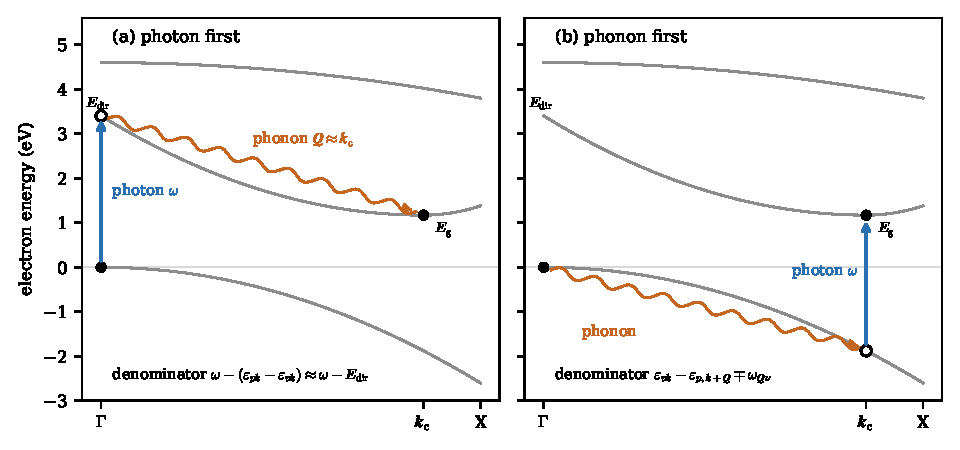
\includegraphics[width=\linewidth]{figures/ch06/fig6_7.pdf}
  \caption{The two time orderings of phonon-assisted absorption across the indirect gap of silicon, on schematic bands along $\mathrm{\Gamma}$--X. Filled dots: the initial electron at the valence maximum at $\mathrm{\Gamma}$ and the final electron at the conduction minimum near $\vect{k}_{\mathrm{c}} = 0.85\,(2\pi/a)$, \SI{1.17}{eV} higher. Open dots: virtual intermediate states. Straight arrows: the vertical optical vertex $\hat{\vect{e}}_\gamma\cdot\vect{v}$; wavy arrows: the electron--phonon vertex $g$, which changes the crystal momentum by $\vect{Q} \approx \vect{k}_{\mathrm{c}}$ and the energy by just $\pm\omega_{\vect{Q}\nu}$, tens of meV. Energy is not conserved at the intermediate state; each panel gives the energy denominator with which its amplitude enters \cref{eq:6.5-M}. (a) Photon first: the intermediate electron is at $\mathrm{\Gamma}$, and the denominator vanishes when $\omega$ reaches the vertical gap $E_{\mathrm{dir}} = \SI{3.4}{eV}$. (b) Phonon first: the intermediate state is a valence state at $\vect{k}_{\mathrm{c}}$, which is occupied. The process then runs through hole orderings, in which an electron from an occupied band is promoted first and the valence electron fills the hole it leaves (sign $-1$), and the denominator of these orderings never vanishes. Band curves drawn by hand; only $\Eg$, $E_{\mathrm{dir}}$ and $\vect{k}_{\mathrm{c}}$ are measured values.}
  \label{fig:6-orderings}
\end{figure}

On the energy shell, $\omega = \varepsilon_{c,\vect{k}+\vect{Q}} - \varepsilon_{v\vect{k}} \pm \omega_{\vect{Q}\nu}$, the denominator of path 3 becomes $\varepsilon_{p,\vect{k}+\vect{Q}} - \varepsilon_{v\vect{k}} \pm \omega_{\vect{Q}\nu}$, and its term takes the form of path 2 with an occupied $p$. The denominator of path 4 becomes $\varepsilon_{p\vect{k}} - \varepsilon_{v\vect{k}} - \omega$, and its term takes the form of path 1 with an occupied $p$. The fermion sign of the hole paths is what makes their terms match the electron paths. The four paths therefore combine into a single one-electron amplitude, summed over every band $p$, occupied or empty:
\begin{equation}
  M^{\pm}_{cv\nu}(\vect{k},\vect{Q}) = \sum_p\left[\frac{g_{cp\nu}(\vect{k},\vect{Q})\;\hat{\vect{e}}_\gamma\cdot\vect{v}_{pv}(\vect{k})}{\omega - \varepsilon_{p\vect{k}} + \varepsilon_{v\vect{k}}} + \frac{\hat{\vect{e}}_\gamma\cdot\vect{v}_{cp}(\vect{k}+\vect{Q})\;g_{pv\nu}(\vect{k},\vect{Q})}{\varepsilon_{v\vect{k}} - \varepsilon_{p,\vect{k}+\vect{Q}} \mp \omega_{\vect{Q}\nu}}\right] .
  \label{eq:6.5-M}
\end{equation}
The sum includes $p = v$ and $p = c$, in which the photon acts as an intraband velocity and the phonon does all the interband work. Refs.~\cite[Eq.~(200)]{giustino2017electron} and~\cite[Eqs.~(2) and~(3)]{noffsinger2012phonon} write the same sum with both denominators of opposite sign, a change that leaves $|M^\pm|^2$ unchanged. Note that the phonon energy enters twice: in the denominator of the phonon-first term, where against electronic energies of electronvolts it is usually negligible, and in the energy balance $\omega = \varepsilon_{c,\vect{k}+\vect{Q}} - \varepsilon_{v\vect{k}} \pm \omega_{\vect{Q}\nu}$, where it shifts the threshold.

A rough size of the amplitude follows from \cref{eq:6.5-M} before any calculation. Compared to a direct transition with a velocity matrix element of similar size, the phonon-assisted amplitude carries an extra factor of the vertex over a denominator. Typical optical-phonon vertices in silicon are a few tenths of an eV (\cref{sec:6.2}) and the denominators near the silicon edge are 2 to \SI{3}{eV}; together they put $|M^\pm|^2$ at $\sim10^{-2}$ of the squared optical vertex for each phonon mode that couples. The phonon-assisted $\varepsilon_2$ near the indirect edge is then $\sim10^{-2}$ of the direct one above $E_{\mathrm{dir}}$, before phase space and occupations are counted. This factor of $\sim10^{-2}$ is why silicon absorbs weakly between its two gaps, and why, for dark matter, the phonon-assisted rate dominates only where the zero-phonon rate is kinematically forbidden.

The photon-first denominator vanishes when $\omega = \varepsilon_{p\vect{k}} - \varepsilon_{v\vect{k}}$, that is, when the photon alone could create a real pair at $\vect{k}$. In silicon the denominator first vanishes at $E_{\mathrm{dir}}$. There the intermediate electron becomes real, and \cref{sec:2.4} gives the treatment. A real electron decays, by phonon emission among other channels, with a width $\varGamma_{\mathrm{w}}$ (\cref{sec:6.3}), and the denominator acquires $+\ii\varGamma_{\mathrm{w}}/2$ (\cref{eq:2.4-width}). By \cref{eq:2.4-split} the squared resonant term then splits into an on-shell part and a finite part. The on-shell part is a cascade: direct absorption at $\vect{k}$, followed by the scattering of the real electron by a phonon, weighted by the branching ratio of the phonon scattering. Direct absorption already counts the cascade once, in \cref{eq:6.5-eps2dir} with a broadened delta function. Adding the full phonon-assisted $\varepsilon_2$ to the direct one above $E_{\mathrm{dir}}$ counts the cascade twice. Below $E_{\mathrm{dir}}$ the double counting does not arise: every intermediate state is off shell, by electronvolts at the indirect edge. First-principles calculations in silicon give the intermediate states a constant width of \SI{100}{meV} and find the spectrum between the gaps insensitive to this width~\cite{noffsinger2012phonon}; the insensitivity is the numerical form of the statement that every intermediate state is off shell.

\subsection{The phonon-assisted dielectric function}

The rest of the derivation is bookkeeping, done as for \cref{eq:6.5-eps2dir}: $T_{fi}$ goes into the rate, the rate into the absorbed power, and the power into $\varepsilon_2$. Summing over the final states, labeled by $\vect{k}$, $\vect{Q}$, $\nu$, $c$, $v$, the spin and the sign, we obtain
\begin{keyresult}[Phonon-assisted dielectric function]
\begin{equation}
  \varepsilon_2^{\mathrm{PA}}(\omega) = \frac{g_{\mathrm{deg}}\,\pi e^2}{\omega^2\,\Omega}\,\Bigl\langle\!\Bigl\langle\sum_{\nu}\sum_{cv}\sum_\pm\bigl(n_{\vect{Q}\nu} + \tfrac12 \pm \tfrac12\bigr)\,\bigl|M^{\pm}_{cv\nu}(\vect{k},\vect{Q})\bigr|^2\,\delta\bigl(\varepsilon_{c,\vect{k}+\vect{Q}} - \varepsilon_{v\vect{k}} \pm \omega_{\vect{Q}\nu} - \omega\bigr)\Bigr\rangle\!\Bigr\rangle ,
  \label{eq:6.5-eps2PA}
\end{equation}
\end{keyresult}
where $\langle\!\langle\cdots\rangle\!\rangle$ is the average over the electron wavevector $\vect{k}$ and the phonon wavevector $\vect{Q}$ in the zone of \cref{eq:A.3-BZ}, and $g_{\mathrm{deg}} = 2$ counts the spin. The formula holds for $T \ll \Eg$, where thermally excited pairs, which would run the process backwards, are absent. Together with \cref{eq:6.5-alpha}, \cref{eq:6.5-eps2PA} gives the absorption coefficient used in first-principles work. Ref.~\cite[Eq.~(1)]{noffsinger2012phonon} writes it in Gaussian units, $e_{\mathrm{G}}^2 = e^2/4\pi$ (\cref{app:A.2}), with the spin factor explicit, and Ref.~\cite[Eq.~(200)]{giustino2017electron} writes it with the spin sum implicit. \Cref{eq:6.5-eps2PA} adds to the direct $\varepsilon_2$ of \cref{eq:6.5-eps2dir}, and below $E_{\mathrm{dir}}$ it is the whole absorption.

The formula contains three sums, and each sets a cost. The sum over intermediate bands $p$, inside $M^\pm$, runs over occupied and empty bands alike, and it converges no faster than its denominators grow; a calculation must include bands several electronvolts above the conduction minimum. The sum over phonon branches is short, six in silicon. The average over $\vect{k}$ and $\vect{Q}$ is the expensive one. The two wavevectors range independently over the whole zone, linked by the energy delta function alone, and the onset region needs both on fine grids. An energy resolution of \SI{14}{meV} in silicon took $40^3$ points for each, $4\times10^9$ pairs, each with its own vertices for every pair of bands~\cite{noffsinger2012phonon}.

In practice no calculation computes so many vertices directly. The energies, velocities and vertices are computed by density-functional perturbation theory on coarse grids, rotated to Wannier functions, and interpolated to the fine grids, with every quantity in one gauge (\cref{sec:6.2}). Two corrections enter the optical vertex. With a nonlocal pseudopotential the velocity includes the commutator of the nonlocal part (\cref{eq:3.2-dHk}), and when the gap is corrected the velocities are rescaled by the ratio of corrected to Kohn--Sham transition energies (\cref{eq:E.3-vrescale}). A different route avoids the double sum altogether. Freezing the nuclei of a supercell in a special displaced configuration breaks translation symmetry; the photon then connects states of different crystal momentum, and one static calculation of $\varepsilon_2$ in that supercell contains the phonon-assisted absorption at a given temperature (\cref{sec:6.3}). Being adiabatic, the special-displacement calculation does not distinguish the emission of a phonon from its absorption, and it cannot resolve the two thresholds $\Eg \pm \omega_{\vect{Q}\nu}$ that the next subsection derives.

\subsection{The Hall--Bardeen--Blatt edge}

Just above the threshold, \cref{eq:6.5-eps2PA} simplifies enough to be done by hand. The final hole lies near the valence maximum at $\vect{k} = 0$, and the final electron near one of the conduction minima $\vect{k}_{\mathrm{c}}$. We measure their crystal momenta from the extrema, $\vect{k} = \vect{\kappa}_{\mathrm{h}}$ and $\vect{k} + \vect{Q} = \vect{k}_{\mathrm{c}} + \vect{\kappa}_{\mathrm{e}}$, and take the bands as parabolic, with kinetic energies $E_{\mathrm{h}} = \kappa_{\mathrm{h}}^2/2m_{\mathrm{h}}$ and $E_{\mathrm{e}} = \kappa_{\mathrm{e}}^2/2m^*_{\mathrm{d}}$. Here $m_{\mathrm{h}}$ is the mass of one valence band and $m^*_{\mathrm{d}} = (m^*_\parallel m^{*2}_\perp)^{1/3}$ the density-of-states mass of one valley, $0.322\,m_e$ in silicon with the valley masses of \cref{tab:3-materials}. Two approximations make the sums elementary. First, the phonon wavevector $\vect{Q} = \vect{k}_{\mathrm{c}} + \vect{\kappa}_{\mathrm{e}} - \vect{\kappa}_{\mathrm{h}}$ stays within the small pockets around $\vect{k}_{\mathrm{c}}$, and the phonon energies and vertices may be taken at $\vect{Q} = \vect{k}_{\mathrm{c}}$; we write $\omega_\nu \equiv \omega_{\vect{k}_{\mathrm{c}}\nu}$ and $n_\nu = n_{\mathrm{B}}(\omega_\nu)$. Second, the denominators of \cref{eq:6.5-M} are electronic energy differences of an electronvolt or more, far from any resonance, and they barely change across the pockets. The squared amplitude $|M^\pm|^2$ is then a constant, its value $|M^\pm_\nu|^2$ at the extrema.

Then only phase space remains. The averages over $\vect{k}$ and $\vect{Q}$ become independent integrals over $\vect{\kappa}_{\mathrm{h}}$ and $\vect{\kappa}_{\mathrm{e}}$, each of which turns into an energy integral with the density of states of a parabolic band, $\int\dd^3\kappa\,(2\pi)^{-3} = \int\dd E\,(2m)^{3/2}E^{1/2}/4\pi^2$. The delta function fixes $E_{\mathrm{e}} + E_{\mathrm{h}} = x$, the energy above the threshold, and
\begin{equation}
  \begin{aligned}
  \Omega^2\!\int\!\frac{\dd^3\kappa_{\mathrm{h}}}{(2\pi)^3}\frac{\dd^3\kappa_{\mathrm{e}}}{(2\pi)^3}\,\delta(x - E_{\mathrm{e}} - E_{\mathrm{h}})
  &= \frac{\Omega^2\,(2m^*_{\mathrm{d}})^{3/2}(2m_{\mathrm{h}})^{3/2}}{16\pi^4}\int_0^x\dd E_{\mathrm{e}}\,E_{\mathrm{e}}^{1/2}(x - E_{\mathrm{e}})^{1/2}\\
  &= \frac{\Omega^2\,(m^*_{\mathrm{d}}m_{\mathrm{h}})^{3/2}}{16\pi^3}\,x^2 ,
  \end{aligned}
  \label{eq:6.5-joint}
\end{equation}
for $x \ge 0$, since the last integral is $\pi x^2/8$. Two densities of states, each growing as $\varepsilon^{1/2}$, have a convolution that grows as $x^2$. A direct edge has one free momentum, because the photon ties the electron to the hole, and its joint density of states grows as $x^{1/2}$; the phonon frees the second momentum and adds a power $3/2$. With all factors collected, each valley, valence band and branch adds a term
\begin{keyresult}[Hall--Bardeen--Blatt edge]
\begin{equation}
  \begin{aligned}
  \alpha_{\mathrm{abs}}(\omega) \simeq \sum_\nu A_\nu\Bigl[&n_\nu\,(\omega - \Eg + \omega_\nu)^2\,\Theta(\omega - \Eg + \omega_\nu)\\
  &+ (n_\nu + 1)\,(\omega - \Eg - \omega_\nu)^2\,\Theta(\omega - \Eg - \omega_\nu)\Bigr] ,
  \end{aligned}
  \label{eq:6.5-edge}
\end{equation}
\end{keyresult}
with
\begin{equation*}
  A_\nu = \frac{g_{\mathrm{deg}}\,e^2\,\Omega\,(m^*_{\mathrm{d}}m_{\mathrm{h}})^{3/2}}{16\pi^2\,\omega\,n_r}\,\sum_{\text{valleys}}|M_\nu|^2 ,
\end{equation*}
constant across the edge. In $A_\nu$ we have set $|M^+_\nu| = |M^-_\nu| \equiv |M_\nu|$, which holds when $\omega_\nu$ is negligible in the denominators, and treated $\omega$ and $n_r$ as constant over the width of the edge, a few times $\omega_\nu$ or about \SI{0.1}{eV}. Heavy and light holes enter as separate valence bands, each with its own $m_{\mathrm{h}}$. \Cref{eq:6.5-edge} is the form of Hall, Bardeen and Blatt~\cite{hall1954infrared}.

\Cref{eq:6.5-edge} turns the edge into a spectroscopy. Each branch that couples contributes two components with the same coefficient $A_\nu$: one starting at $\Eg - \omega_\nu$, where the photon is helped by a phonon absorbed from the lattice, and one at $\Eg + \omega_\nu$, where a phonon is emitted. The midpoint of each pair of thresholds is $\Eg$, and their separation is $2\omega_\nu$. Each component is a straight line in a plot of $\sqrt{\alpha_{\mathrm{abs}}}$ against $\omega$, with slope $\sqrt{A_\nu n_\nu}$ or $\sqrt{A_\nu(n_\nu + 1)}$. The sum of several components is not a straight line, and the measured curve is decomposed by subtracting, at each threshold, the extrapolation of the components that started below it.

The quadratic law assumes that $M_\nu$ is finite at the extrema, that is, that the transition is \emph{allowed} there. If symmetry forces $M_\nu$ to vanish at the extrema, it grows linearly with $\kappa_{\mathrm{e}}$ or $\kappa_{\mathrm{h}}$, an extra power of energy enters the integrand of \cref{eq:6.5-joint}, and the forbidden edge grows as $x^3$. The quadratic law also neglects the attraction between the electron and the hole. In silicon the bound pair, the exciton, lies $E_x^b = \SI{14.7}{meV}$ below the gap at total crystal momentum $\vect{k}_{\mathrm{c}}$ (\cref{sec:4.9}), and a photon reaches the exciton with a phonon just as it reaches a free pair. Each threshold of \cref{eq:6.5-edge} therefore has an excitonic companion $E_x^b$ lower, with its own onset shape, and the kinks of a measured edge are exciton thresholds at $\Eg - E_x^b \pm \omega_\nu$.

\subsection{Temperature dependence}

All of the temperature dependence of \cref{eq:6.5-edge} at a fixed gap is in the occupations. The component that absorbs a phonon is proportional to $n_\nu$, the number of phonons available; the one that emits is proportional to $n_\nu + 1$, spontaneous plus stimulated emission. Their ratio,
\begin{equation}
  \frac{n_\nu}{n_\nu + 1} = \ee^{-\omega_\nu/T} ,
  \label{eq:6.5-ratio}
\end{equation}
is detailed balance (\cref{eq:2.5-db}) for the phonon system alone: the two components have the same $|M_\nu|^2$, and the lattice gives up an energy $\omega_\nu$ with a Boltzmann penalty relative to taking it. The ratio of the slopes of the two components in $\sqrt{\alpha_{\mathrm{abs}}}$ is $\ee^{-\omega_\nu/2T}$, and the edge is a thermometer of the lattice that needs no knowledge of $A_\nu$. At high temperature both components grow as $T/\omega_\nu$, and the total weight of a branch, proportional to $2n_\nu + 1$, rises with $T$.

As $T \to 0$ the absorption components vanish. A cold crystal has no phonons to give, and every photon absorbed at the indirect edge must create one. The edge then lies at $\Eg + \omega_\nu$ for the softest branch that couples, and the energy $\omega_\nu$ of the emitted phonon goes into the lattice, not into the pair. At the \SI{10}{mK} of a dark-matter detector the emission-only edge is exact for every practical purpose: the transverse-acoustic occupation in silicon is vanishingly small (\cref{we:6-siedge}).

The gap itself also moves with temperature. The phonon-assisted formula contains the occupations explicitly; the bands in \cref{eq:6.5-eps2PA} are the bands the electrons actually occupy, renormalized by the same electron--phonon coupling (\cref{sec:6.3}). In silicon the gap shrinks from \SI{1.17}{eV} at low temperature to \SI{1.12}{eV} at \SI{300}{K} (\cref{sec:3.3}), and all four thresholds of each branch move down with it. First-principles spectra that include the occupations alone must be shifted rigidly to match the measured onsets, by 0.15 to \SI{0.23}{eV} in silicon, a shift that absorbs both the remaining error of the computed gap and the electron--phonon renormalization of the gap~\cite{noffsinger2012phonon}.

\subsection{The silicon edge}

Macfarlane, McLean, Quarrington and Roberts measured the absorption edge of silicon between \SI{4.2}{} and \SI{415}{K}, with enough resolution to see the thresholds of \cref{eq:6.5-edge}~\cite{macfarlane1958fine}. They found four series of thresholds and quoted the phonon energies as temperatures $\theta$, which in natural units are the energies themselves. Two of these phonon energies, $\theta = \SI{212}{K}$ and \SI{670}{K}, belong to the transverse-acoustic and transverse-optical phonons at $\vect{k}_{\mathrm{c}}$~\cite[Chap.~6]{yu2010fundamentals}. With $\SI{1}{K} = \SI{86.17}{\micro eV}$ (\cref{sec:2.5}) the two energies are
\begin{equation*}
  \omega_{\mathrm{TA}} = \SI{18.27}{meV}, \qquad \omega_{\mathrm{TO}} = \SI{57.73}{meV} .
\end{equation*}
Neutron scattering measures the same branches at the zone boundary X, at \SI{4.49}{THz} and \SI{13.90}{THz}, or \SI{18.57}{meV} and \SI{57.49}{meV} (\cref{sec:5.2}). Both branches are flat between $\vect{k}_{\mathrm{c}} = 0.85\,\mathrm{X}$ and X: in the computed dispersion of \cref{sec:5.2} they change by \SI{0.1}{\percent} (TA) and \SI{0.3}{\percent} (TO) over that interval. The optical and the neutron values measure the same phonons, and they agree to \SI{2}{\percent} for the transverse-acoustic branch and to \SI{0.4}{\percent} for the transverse-optical one. The measured thresholds were exciton thresholds, a binding energy below the free-pair ones, as \cref{sec:4.9} anticipated.

\Cref{fig:6-edge} shows \cref{eq:6.5-edge} with these energies. Panel (b) separates the four components at \SI{300}{K} and shows that each is a straight line in $\sqrt{\alpha_{\mathrm{abs}}}$ with its own threshold, while their sum bends at every threshold. Panel (a) follows the sum down in temperature. The components that absorb a phonon fade first, the transverse-optical one long before the transverse-acoustic one, and at \SI{77}{K} the edge is already dominated by emission.

\begin{figure}[tbp]
  \centering
  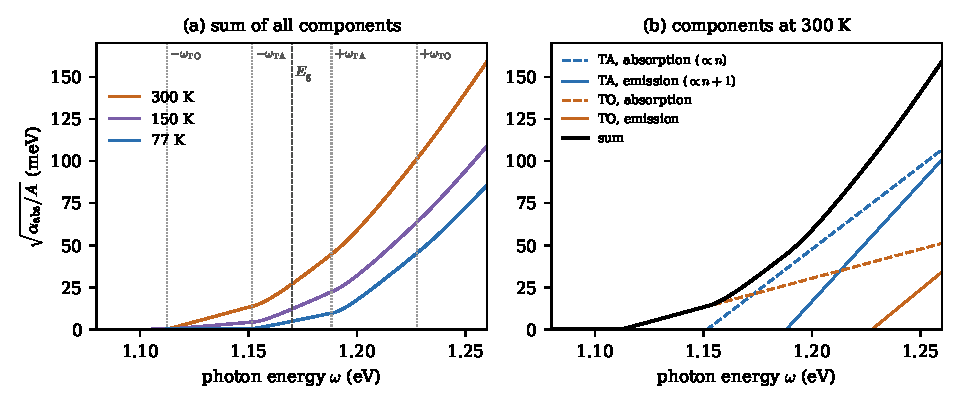
\includegraphics[width=\linewidth]{figures/ch06/fig6_8.pdf}
  \caption{The Hall--Bardeen--Blatt edge of silicon, \cref{eq:6.5-edge}, plotted as $\sqrt{\alpha_{\mathrm{abs}}/A}$ against the photon energy, with $\Eg = \SI{1.17}{eV}$ and the phonon energies $\omega_{\mathrm{TA}} = \SI{18.27}{meV}$ and $\omega_{\mathrm{TO}} = \SI{57.73}{meV}$ measured from the optical edge~\cite{macfarlane1958fine}. Dotted lines mark the free-pair thresholds $\Eg \mp \omega_{\mathrm{TO}}$ and $\Eg \mp \omega_{\mathrm{TA}}$; the dashed line marks $\Eg$, their common midpoint. (a) Sum of the four components at \SI{300}{K}, \SI{150}{K} and \SI{77}{K}. (b) The components at \SI{300}{K}: dashed, phonon absorption, proportional to $n_\nu$; solid, phonon emission, proportional to $n_\nu + 1$. Each component is a straight line; the sum (black) is not. The two branches are given equal coefficients $A_{\mathrm{TA}} = A_{\mathrm{TO}} = A$, so their relative heights are illustrative. The gap is held at its low-temperature value at every temperature, to isolate the phonon occupations (\cref{sec:6.3} treats its shift). The excitonic thresholds, \SI{14.7}{meV} lower, are omitted.}
  \label{fig:6-edge}
\end{figure}

\begin{workedexample}{The phonon thresholds of silicon}\label{we:6-siedge}
With $\Eg = \SI{1.17}{eV}$ and the phonon energies above, the four free-pair thresholds of \cref{eq:6.5-edge} are
\begin{equation*}
  \begin{gathered}
  \Eg - \omega_{\mathrm{TO}} = \SI{1.1123}{eV}, \qquad
  \Eg - \omega_{\mathrm{TA}} = \SI{1.1517}{eV}, \\
  \Eg + \omega_{\mathrm{TA}} = \SI{1.1883}{eV}, \qquad
  \Eg + \omega_{\mathrm{TO}} = \SI{1.2277}{eV} .
  \end{gathered}
\end{equation*}
The exciton binding $E_x^b = \SI{14.7}{meV}$ moves each of them down by that amount. The pairs of thresholds are symmetric about $\Eg$, separated by $2\omega_{\mathrm{TA}} = \SI{36.5}{meV}$ and $2\omega_{\mathrm{TO}} = \SI{115.5}{meV}$.

The slopes depend on the occupations alone, not on the gap. At \SI{300}{K}, $T = \SI{25.85}{meV}$, and
\begin{equation*}
  n_{\mathrm{TA}} = \frac{1}{\ee^{18.27/25.85} - 1} = 0.973, \qquad n_{\mathrm{TO}} = \frac{1}{\ee^{57.73/25.85} - 1} = 0.120 .
\end{equation*}
In units of $\sqrt{A_\nu}$, the transverse-acoustic components of $\sqrt{\alpha_{\mathrm{abs}}}$ rise with slopes $\sqrt{n_{\mathrm{TA}}} = 0.987$ (absorption) and $\sqrt{n_{\mathrm{TA}} + 1} = 1.405$ (emission), the transverse-optical ones with 0.346 and 1.058. The ratios of the slopes in each pair, 0.702 and 0.327, are $\ee^{-\omega_\nu/2T}$ for the two branches, independent of $A_\nu$. Read backwards, the transverse-acoustic ratio gives $-2T\ln 0.702 = \SI{18.27}{meV}$: the slope ratio of one branch returns its phonon energy if the temperature is known, or the temperature if the phonon energy is. At \SI{77}{K}, $T = \SI{6.635}{meV}$, the occupations fall to $n_{\mathrm{TA}} = 0.068$ and $n_{\mathrm{TO}} = 1.7\times10^{-4}$, and the slope ratios to 0.252 and 0.013. At \SI{20}{K} the transverse-acoustic absorption component has $n_{\mathrm{TA}} = 2.5\times10^{-5}$, and at the \SI{10}{mK} of a cryogenic detector $\omega_{\mathrm{TA}}/T = 2.1\times10^4$: the occupation is $\ee^{-21200}$, and only the emission thresholds exist. The lowest of them is the true optical edge of cold silicon, \SI{18}{meV} above the gap. With the measured low-temperature gap $\Eg(0) = \SI{1.1692}{eV}$ of \cref{sec:6.3} in place of the rounded value, this edge lies at $\Eg(0) + \omega_{\mathrm{TA}} = \SI{1.1875}{eV}$ for a free pair, and the excitonic edge at \SI{1.1728}{eV}, since $\omega_{\mathrm{TA}}$ and $E_x^b$ nearly cancel.
\end{workedexample}

\subsection{Phonon-assisted dark-matter scattering}

The derivation of \cref{eq:6.5-M} used only two properties of the photon: it couples to the electrons through a one-body operator, and it carries negligible momentum. A dark-matter particle that interacts with the electron density keeps the first property and loses the second. Its vertex is the dark-matter potential $\tilde V(\vect{q})$ times the matrix element of $n_e(\vect{q}) = \int\dd^3r\,\ee^{\ii\vect{q}\cdot\vect{r}}\,\op{\nd}_e(\vect{r})$, the Fourier component of the density operator. Between Bloch states this matrix element is the density vertex $\rho_{mn}(\vect{k},\vect{q})$ of \cref{eq:3.2-rho}. The optical vertex $\hat{\vect{e}}_\gamma\cdot\vect{v}_{pv}(\vect{k})$ is replaced by $\rho_{pv}(\vect{k},\vect{q})$, which is no longer vertical: it takes the electron from $\vect{k}$ to $\vect{k} + \vect{q}$. The phonon then supplies the rest of the crystal momentum, $\vect{Q} = \vect{k}_{\mathrm{c}} - \vect{q}$ up to a reciprocal-lattice vector for a transition from the valence maximum to a valley. The amplitude has the same orderings and the same hole paths, but its vertices and energies are evaluated at three crystal momenta, $\vect{k}$, $\vect{k} + \vect{q}$ and $\vect{k} + \vect{q} + \vect{Q}$, instead of two.

The energy denominators take the energy deposited $\omega$ in place of the photon energy, and they resonate wherever $\omega$ matches a real pair at momentum transfer $\vect{q}$, with the same risk of double counting as at $E_{\mathrm{dir}}$. Since $\rho_{mn}$ reduces to the optical vertex as $q \to 0$ (\cref{eq:3.2-optical}), the measured silicon edge is the zero-momentum limit of the dark-matter amplitude and a test of any calculation of it.

Absorbed bosons and scattering particles meet this amplitude in different limits. An absorbed boson, a kinetically mixed dark photon for instance, deposits its whole mass with a momentum $m_\phi v \approx 10^{-3}m_\phi$, a smaller momentum for its energy than a photon carries. Its absorption between $\Eg$ and $E_{\mathrm{dir}}$ is \cref{eq:6.5-eps2PA} with the photon's coupling replaced by its own and screened by the medium (\cref{sec:8.4-mixing}). A scattering particle transfers $\vect{q}$ and $\omega$ together, with $\omega \le qv_{\mathrm{max}} - q^2/2\mchi$ (\cref{eq:1.3-region}). Far above its threshold mass it reaches $\vect{k}_{\mathrm{c}}$ at first order, but just above the threshold mass the energy needed to cross the gap is available at momentum transfers well below $k_{\mathrm{c}}$, where the zero-phonon transition is forbidden (\cref{sec:3.3}). At the threshold mass, $\omega = \Eg$ is reached just at $q = 2\Eg/v_{\mathrm{max}} = \SI{0.88}{keV}$, and for heavier dark matter the smallest such $q$ falls toward $\Eg/v_{\mathrm{max}} = \SI{0.44}{keV}$; both lie well below $k_{\mathrm{c}} = 0.85\,(2\pi/a) = \SI{1.9}{keV}$. At these momentum transfers, as for light below $E_{\mathrm{dir}}$, the phonon-assisted amplitude is the leading process, and it opens a window of masses in which silicon sees dark matter only through the phonon-assisted process. In a cold detector, however, only the emission branch contributes: the phonon takes part of the energy deposited, and the pair receives $\omega - \omega_{\vect{Q}\nu}$.

\section*{Summary}

The Born--Oppenheimer approximation keeps only the diagonal of the coupling between electrons and nuclei, and the off-diagonal coupling follows from the derivative-coupling vector $\vect{d}_{ji} = \langle\Psi_j|\nabla\Psi_i\rangle$ (\cref{sec:6.1}). To first order in the displacements the same physics is the electron--phonon Hamiltonian $H_{\mathrm{ep}}$, in which a phonon of wavevector $\vect{Q}$ moves an electron from $\vect{k}$ to $\vect{k} + \vect{Q}$ with the vertex $g_{mn\nu}(\vect{k},\vect{Q})$. Whether the electrons follow a moving nucleus depends on how fast the nucleus is accelerated. If the acceleration is slow compared with $1/\Delta E$, the electrons stay in their ground state. If it is sudden, they keep their state while the nucleus acquires a velocity $v_N$, and the complement of the overlap of the boosted ground state with the original one is the Migdal effect.

The vertex that density-functional perturbation theory computes is screened (\cref{sec:6.2}). Acoustic phonons couple through deformation potentials, with $g \propto Q^{1/2}$, optical phonons in nonpolar crystals through optical deformation potentials, and longitudinal optical phonons in polar crystals through the Fr\"ohlich vertex $g^{\mathrm{L}} = \ii C_{\mathrm{F}}\rho_{mn}/Q$, which in GaAs gives a polaron constant $\alpha_{\mathrm{F}} = 0.072$.

Second order in the displacements yields the electron self-energy, the Fan--Migdal and Allen--Heine terms, which in the adiabatic limit combine into the average of the band energy over the zero-point and thermal smearing of the lattice (\cref{sec:6.3}). For the indirect gap of silicon the computed zero-point renormalization is \SI{-56.2}{meV}; the measured electron--phonon part, $-71$ to \SI{-73}{meV}, is about \SI{20}{\percent} larger. A detector at \SI{10}{mK} sees the low-temperature gap, which already contains the full renormalization.

Photons between the indirect gap of silicon and its direct gap of \SI{3.4}{eV} are absorbed only with a phonon (\cref{sec:6.5}). Summed over electron and phonon wavevectors in the whole zone, the squared second-order amplitude $|M^\pm|^2$ gives the phonon-assisted dielectric function $\varepsilon_2^{\mathrm{PA}}$. Near the edge it reduces to the Hall--Bardeen--Blatt law, each phonon branch adding components growing as $(\omega - \Eg \pm \omega_\nu)^2$, and in a cold detector only emission survives. Replacing the optical vertex by the density vertex turns phonon-assisted absorption of light into the phonon-assisted response to dark matter, which governs the absorption of light bosons (\cref{sec:13.8}) and the threshold window of electron recoils in silicon.

A phonon decays into electron--hole pairs only where real pairs exist at its energy (\cref{sec:6.4}). Its self-energy is the electron bubble, whose static part is already contained in the frequencies of density-functional perturbation theory. In a metal the imaginary part leads to Allen's formula, the Eliashberg function $\alpha^2F(\omega)$ and the coupling constant $\lambda_{\mathrm{ep}}$. For aluminum a free-electron model with one core radius yields $\lambda_{\mathrm{ep}} = 0.436$, against 0.42 to 0.43 from tunneling and the specific heat, and $\lambda_{\mathrm{ep}}$ sets the strength of the pairing in the superconducting sensors of \cref{chap:7}.
